% Author: Mick van Gelderen
% Example tikz include file

\documentclass{article}
\usepackage{comment}

\usepackage{tikz}
\usetikzlibrary{calc,positioning,shapes,arrows,decorations.pathreplacing}
\usetikzlibrary{shapes.multipart}


\begin{document}

\begin{figure}[h]
	\centering
	% Author: Mick van Gelderen
% Created from http://www.texample.net/tikz/examples/class-diagram/ and other examples and resources. 

%\documentclass{standalone}
%\usepackage{tikz}
\usetikzlibrary{calc,positioning,shapes,arrows,decorations.pathreplacing}
\usetikzlibrary{shapes.multipart}


%\begin{document}




\newcommand{\activity}[3]{\node (v#1) [activity, text width=#2cm, #3] {$v_#1$};}

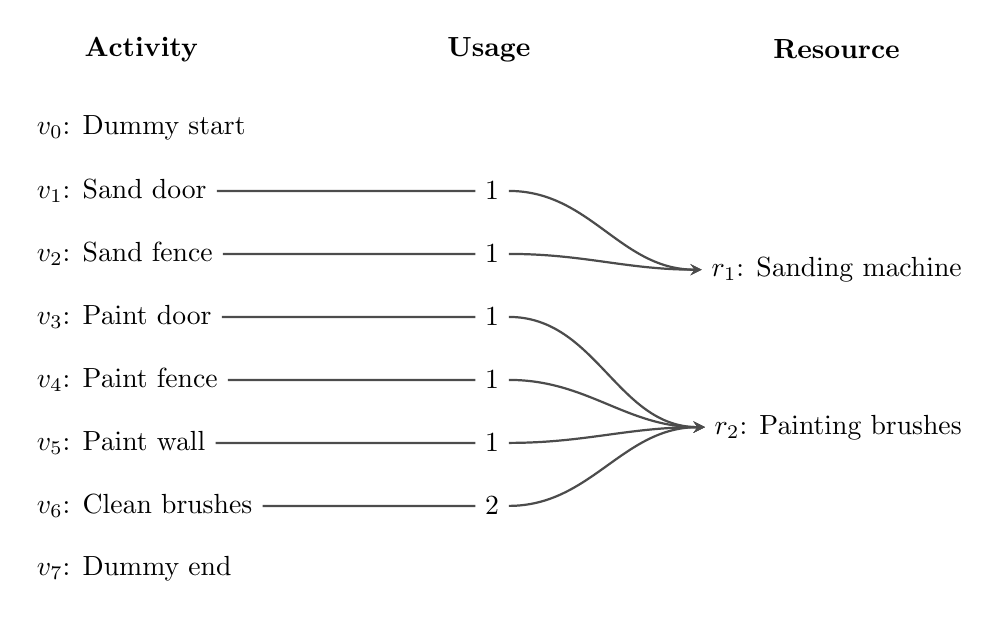
\begin{tikzpicture}[node distance=.8cm]
	\tikzstyle{activity}=[text centered, text=black, thick, minimum height=1.8em, minimum width=1.8em]
	\tikzstyle{resource}=[text centered]
	\tikzstyle{header}=[font=\bfseries]
	\tikzstyle{usage}=[->,>=stealth, draw=black!70, thick]

	\node (v0) [activity] {$v_0$: Dummy start};
	\node (v1) [activity, below=of v0.west, anchor=west] {$v_1$: Sand door};
	\node (v2) [activity, below=of v1.west, anchor=west] {$v_2$: Sand fence};
	\node (v3) [activity, below=of v2.west, anchor=west] {$v_3$: Paint door};
	\node (v4) [activity, below=of v3.west, anchor=west] {$v_4$: Paint fence};
	\node (v5) [activity, below=of v4.west, anchor=west] {$v_5$: Paint wall};
	\node (v6) [activity, below=of v5.west, anchor=west] {$v_6$: Clean brushes};
	\node (v7) [activity, below=of v6.west, anchor=west] {$v_7$: Dummy end};
	
	\node (u1) [right=5.7cm of v1.west] {1};
	\node (u2) [right=5.7cm of v2.west] {1};
	\node (u3) [right=5.7cm of v3.west] {1};
	\node (u4) [right=5.7cm of v4.west] {1};
	\node (u5) [right=5.7cm of v5.west] {1};
	\node (u6) [right=5.7cm of v6.west] {2};

	\coordinate (mid) at ($(v0.west)!.5!(v7.west) + (12,0)$);
	\node (r1) [resource, above=1cm of mid, anchor=east] {$r_1$: Sanding machine};
	\node (r2) [resource, above=-1cm of mid, anchor=east] {$r_2$: Painting brushes};

	\draw let \p1 = (v0), \p2 = (r1) in 
		node (ac) [header] at ($(\x1,\y1) + (0,1)$) {Activity}
		node (res) [header] at ($(\x2,\y1) + (0,1)$) {Resource};
	\node (us) [header] at ($(ac)!.5!(res)$) {Usage};
	
  \draw[usage] (v1.east) -- (u1) to[out=0,in=180] (r1.west);
  \draw[usage] (v2.east) -- (u2) to[out=0,in=180] (r1.west);
  \draw[usage] (v3.east) -- (u3) to[out=0,in=180] (r2.west);
  \draw[usage] (v4.east) -- (u4) to[out=0,in=180] (r2.west);
  \draw[usage] (v5.east) -- (u5) to[out=0,in=180] (r2.west);
  \draw[usage] (v6.east) -- (u6) to[out=0,in=180] (r2.west);

  
	
\end{tikzpicture}

%\end{document}
	\caption{Example of an activity graph with dummy activities. }
	\label{fig:activity_graph}
\end{figure}

\begin{comment}
\begin{center}
% Author: Mick van Gelderen
% Created from http://www.texample.net/tikz/examples/class-diagram/ and other examples and resources. 

%\documentclass{standalone}
%\usepackage{tikz}
\usetikzlibrary{calc,positioning,shapes,arrows,decorations.pathreplacing}
\usetikzlibrary{shapes.multipart}


%\begin{document}

\tikzstyle{activity}=[rectangle, draw=black, text centered, anchor=west, text=black, thick, minimum height=1.8em, minimum width=1.8em]
\tikzstyle{dummy}=[rectangle, draw=black, text centered, anchor=west, text=black, thick, minimum height=1.8em, minimum width=1.8em]
\tikzstyle{precedence}=[->,>=stealth, draw=black!70, thick]

\begin{tikzpicture}[node distance=1]
    \node (v0) [dummy, text width=.5cm] {$v_0$};
    \node (v2) [activity, text width=4cm, right=of v0] {$v_2$};
    \node (v1) [activity, text width=3cm, above=of v2] {$v_1$};
    \node (v3) [activity, text width=2cm, below=of v2] {$v_3$};
    \node (v4) [activity, text width=2cm, right=of v2] {$v_4$};
    \node (v5) [dummy, text width=.5cm, right=of v4] {$v_5$};
    
    \draw[precedence] (v0.east) to[out=0,in=180] (v1.west);
    \draw[precedence] (v0.east) to[out=0,in=180] (v2.west);
    \draw[precedence] (v0.east) to[out=0,in=180] (v3.west);
    \draw[precedence] (v1.east) to[out=0,in=180] (v4.west);
    \draw[precedence] (v2.east) to[out=0,in=180] (v4.west);
    \draw[precedence] (v4.east) to[out=0,in=180] (v5.west);
    % start bending from the projection v4 on the line y=v3.y
    \draw[precedence] (v3.east) -- ($(v3)!(v4)!($(v3)+(1,0)$)$) to[out=0,in=180] (v5.west);

    % Descriptions
    \path (v1.east) to[out=0,in=180] coordinate (temp) (v4.west);
    \draw[shorten <=2pt, shorten >=2pt] (temp) -- ++(.8,.6) node[anchor=west, yshift=2pt] {Precedence constraint $(v_1, v_4) \in E$};
    
    \draw[shorten <=2pt, shorten >=2pt] (v3.south) -- ++(.8,-.6) node[anchor=west, yshift=-2pt] {Activity $v_3$};
    
    % Funky braces
    \draw[decorate,decoration={brace,amplitude=8pt}]
        let \p1 = (v2.west), \p2 = (v4.east), \p3 = (v1) in 
        (\x1, \y3+1cm) -- (\x2, \y3+1cm) node[midway, above=10pt] {$V = \{v_1, \ldots, v_4\}$};
        
    \draw[decorate,decoration={brace,amplitude=8pt}]
        let \p1 = (v0.west), \p2 = (v5.east), \p3 = (v1) in 
        (\x1, \y3+2cm) -- (\x2, \y3+2cm) node[midway, above=10pt] {$W = V \cup \{v_0, v_5\}$};
    
\end{tikzpicture}

%\end{document}
\vspace{1em}
\emph{The activities $v_0$ and $v_5$ are dummy activities. They do not belong to the original set of activities $V$. The set $W$ consists of the original activities plus the dummy activities. }
\end{center}

\vspace{2cm}

\begin{center}
% Author: Mick van Gelderen
% Created from http://www.texample.net/tikz/examples/class-diagram/ and other examples and resources. 

%\documentclass{standalone}
%\usepackage{tikz}
\usetikzlibrary{calc,positioning,shapes,arrows,decorations.pathreplacing}
\usetikzlibrary{shapes.multipart}


%\begin{document}

\tikzstyle{activity}=[rectangle, draw=black, text centered, anchor=south west, text=black, minimum height=1cm, minimum width=1cm]
\tikzstyle{axis}=[->,thick,>=stealth]

\begin{tikzpicture}[node distance=1]
    \draw[axis] (-.5,0) -- (8.5,0) node[anchor=north] {Time};
    \draw[axis] (0,-.5) -- (0,2.5) node[anchor=north east] {Activities} ;
    
    \node (v0) [activity] at (0,0) {$v_0$};
    \node (v2) [activity, minimum width=4cm] at (1,0) {$v_2$};
    \node (v1) [activity, minimum width=3cm] at (1,1) {$v_1$};
    \node (v3) [activity, minimum width=2cm] at (4,1) {$v_3$};
    \node (v4) [activity, minimum width=2cm] at (5,0) {$v_4$};
    \node (v5) [activity] at (7,0) {$v_5$};
    
    \draw[dotted] (v1.south east) -- ++(0,-1) node[anchor=north] {$t_3$};
    \draw[dotted] (v3.south east) -- ++(0,-1) node[anchor=north] {$t_5$};
    \node [anchor=north] at (v2.south west) {$t_0$};
    \node [anchor=north] at (v4.south west) {$t_4$};
    \node [anchor=north] at (v5.south west) {$t_6$};
    
\end{tikzpicture}

%\end{document}
\end{center}
\end{comment}
\end{document}